\chapter{Background} % Main chapter title

\label{Chapter2} % For referencing this chapter elsewhere, use \ref{Chapter2}

\lhead{Chapter 2. \emph{Background}}

%----------------------------------------------------------------------------------------
%	SECTION 2.1 - On Number representation
%----------------------------------------------------------------------------------------

\section{On Number Representation}

The question of the representation of numbers as we, humans, use them in a world of electronics has been central in the creation of computers and their associated arithmetics. Several problems are contained in the simple question of: How to translate our arithmetic and number operations in a piece of hardware?

%-----------------------------------
%	SUBSECTION 2.1.1 - Number Representation
%-----------------------------------
\subsection{Number Representation}

The first thing to note is that electronics can represent two states, a presence or absence of an electric impulsion. The states of \guille{on} and \guille{off} is embedded in transistors that can represent both. The transistor is the hardware representant of this duality while a bit is its software counter-part. This is the underlying reason why computers, even the first fully electronical computer ENIAC (\emph{Electronical Numerical Integrator and Computer}), use a binary system. If this system is handy to translate our base 10 arithmetic and simple numbers such as integers, it is harder to translate more complex numbers such as reals and floating point operations. The meaning of an N-bit binary word is entirely dependent of the interpretation we choose to use. This interpretation consists of both a representation (the type of the object the memory represents) and its associated mapping. Common number representations consists of unsigned integers, signed integers (using two's complement), floating point reals as well as fixed-point reals.

%-----------------------------------
%	SUBSUBSECTION 2.1.1.1 - Integer Representation
%-----------------------------------
\subsubsection{Integer Representation}

The representation of integers and especially unsigned integers is straightforward as it consists of a change form base 10 to base 2. This number representation can be done in 16-bits, 32-bits or 64-bits depending on its type, the supporting hardware and the space we need to contain it. Representing a number in base 2 from base 10 or vice versa is straightforward as it only demands simple and exact basic operations to be performed. As shown on \emph{Figure} \ref{fig:IntegerRepr}, $4576 = 2^5 + 2^6 + 2^7 + 2^8 + 2^{12}$.

Now, if we want to represent a signed integer, we have to use a method called the \emph{two's complement} in order to bring the sign in. This method keeps the basic behaviour of the addition to work on numbers be they positive or negative. The method consists in changing the value of all the bits of a given number then adding one to the result. The representation of -4576 when doing the computation with 13 bits (1 sign bit and 12 mantissa bits) consists of:
\begin{align}
(01000111100000)^\text{two's complement} &= (01000111100000)^\text{one's complement} + 1\\ \nonumber
                                         &= 10111000011111 + 1\\ \nonumber
                                         &= 10111000100000
\end{align}

The result for 32 and 64 bits can be seen on \emph{Figure} \ref{fig:IntegerRepr}.

\begin{figure}[htbp]
	\centering
		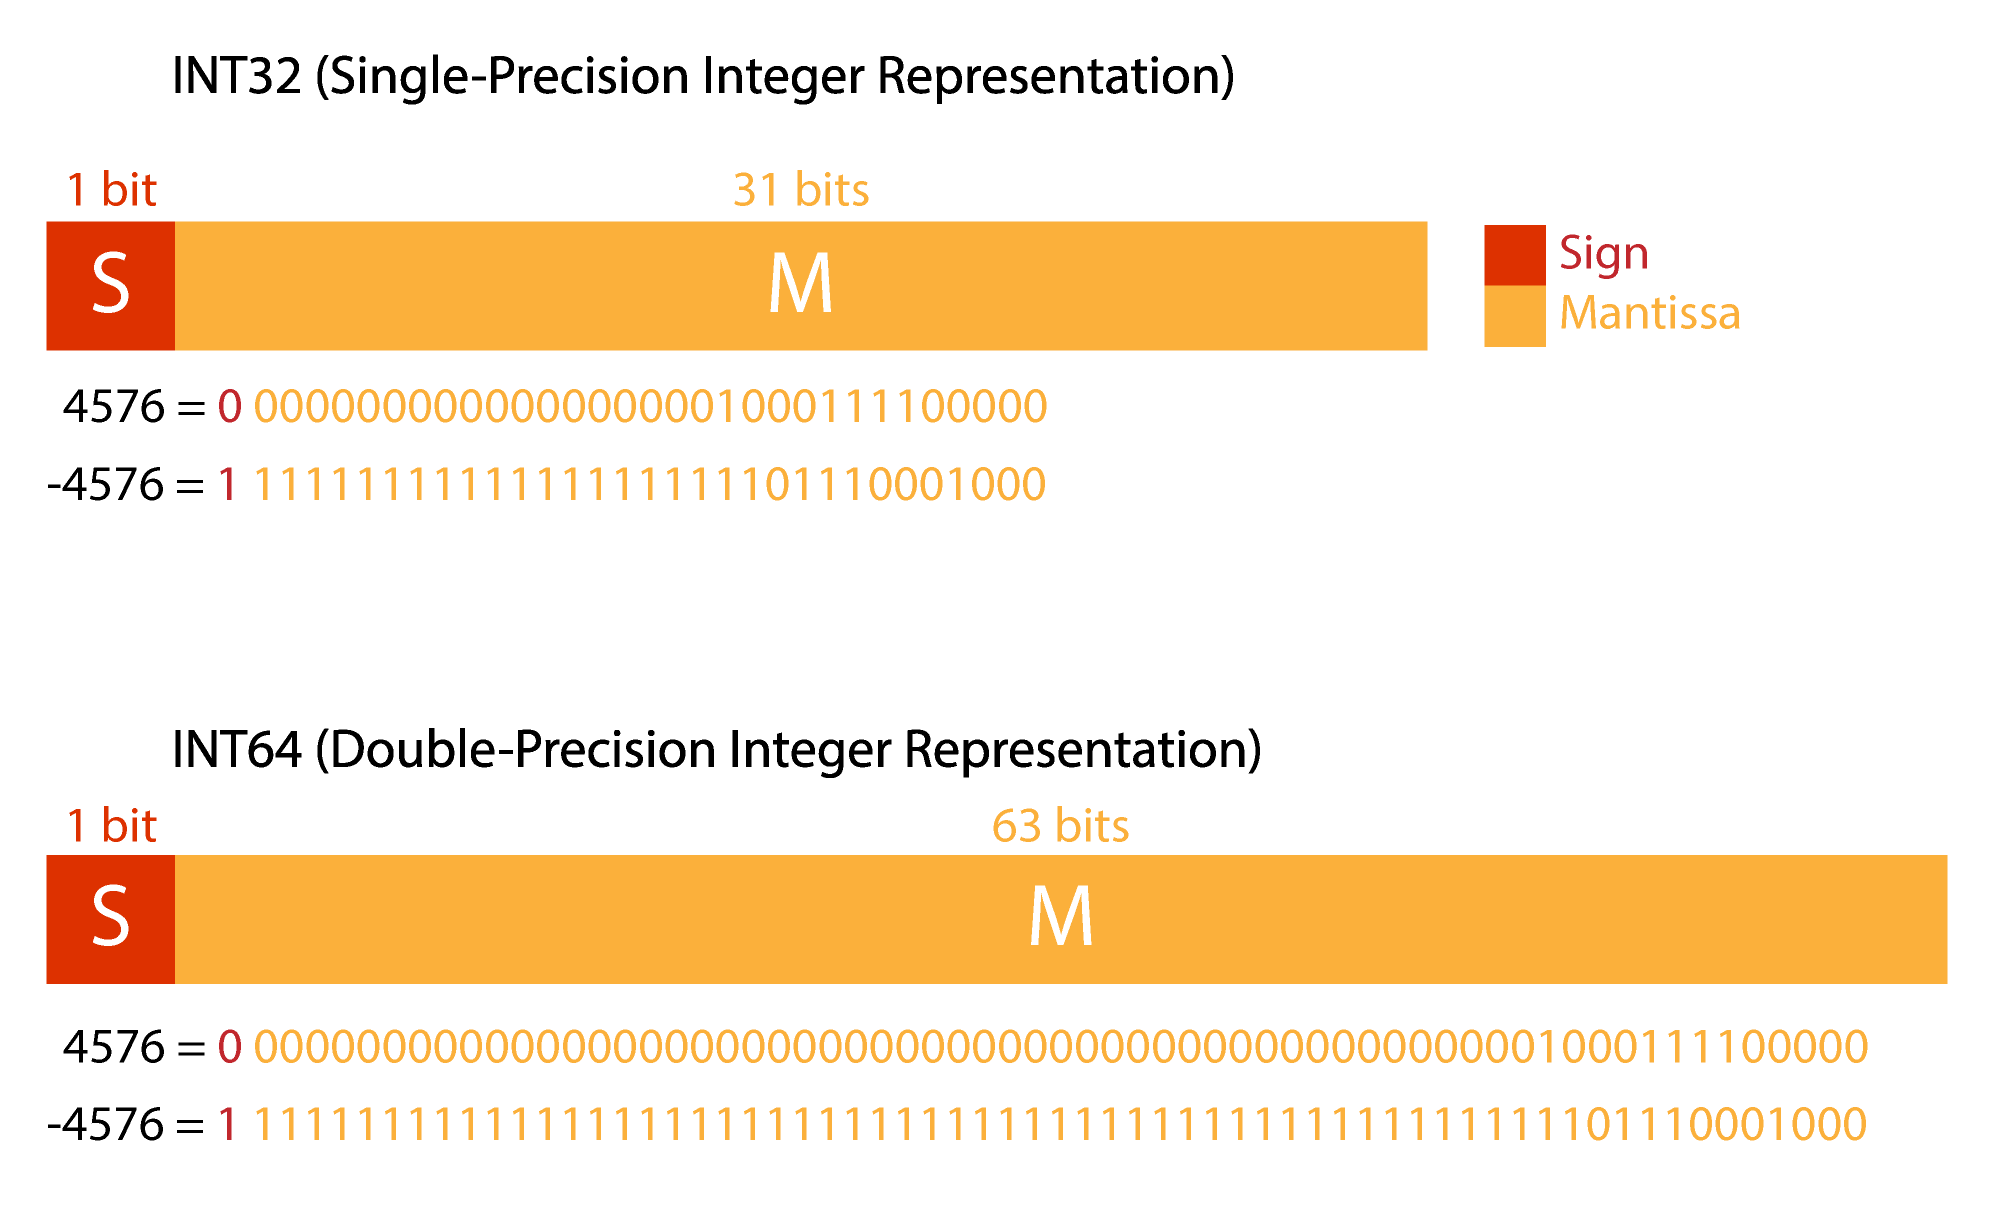
\includegraphics[width=.8\textwidth]{Figures/IntegerRepr.png}
	\caption[Integer Representation]{Integer Representation and Two's Complement example}
	\label{fig:IntegerRepr}
\end{figure}

% TODO CORRECT FIGURE

Those two representations allow a complete mapping of integers up to a certain range: signed 32-bit integers can represent numbers between -2,147,483,648 and 2,147,483,647 while unsigned integers can represent numbers between 0 and 4,294,967,295.

%-----------------------------------
%	SUBSUBSECTION 2.1.1.2 - Floating-Point Representation
%-----------------------------------
\subsubsection{Floating-Point Representation}

Representing floating-point numbers has been a concern since the 1980's and the industrial development of several computing modules and interfaces. The need for a consensus in this domain and particular applications has been answered by the IEEE-754 standard \cite{Ieee754_1985} in 1985. This standard defines both the floating-point number representations and exceptions conditions along with their default handling. This norm was reviewed fundamentally in 2008 \cite{Ieee754_2008}, extending it to 64-bits and 128-bits length. The last dated revision of the norm is from 2019 \cite{Ieee754_2019}.

Floating-point numbers following this representation are composed of three distinct elements:
\begin{enumerate}
  \item A sign bit
  \item An exponent
  \item A mantissa
\end{enumerate}

Those three elements compose the number by using the following formula: $(\mathit{sign}) \times \mathit{mantissa} \times 2^{\mathit{exponent}}$

In order to present both positive and negative exponents and as using the two's complement on the exponent would complexify the computation of floating-point numbers, a bias is used in the exponent. This bias corresponds to $2^e - 1$ where e is the number of bits of the exponent part. This means that with an 8-bit exponent, the bias is equal to 127. An exponent equal to $00000111$ is equal to $7 - 127 = -120$ and an exponent equal to $10000111$ is equal to $135 - 127 = 8$. An 8-bit exponent can cover a range from -126 to 127 (because exponents -127 (all 0s) and +128 (all 1s) are reserved for special numbers.

When referring to single-precision floating-point representation we are talking about 32-bit long memory representation. They are mapped as follows and as shown in \emph{Figure} \ref{fig:FP32}:
\begin{itemize}
  \item Sign bit: 1 bit
  \item Exponent: 8 bits
  \item Mantissa: 23 bits
  \item Exponent Bias: 127
\end{itemize}

% FP32 EXAMPLE
\begin{figure}[htbp]
	\centering
		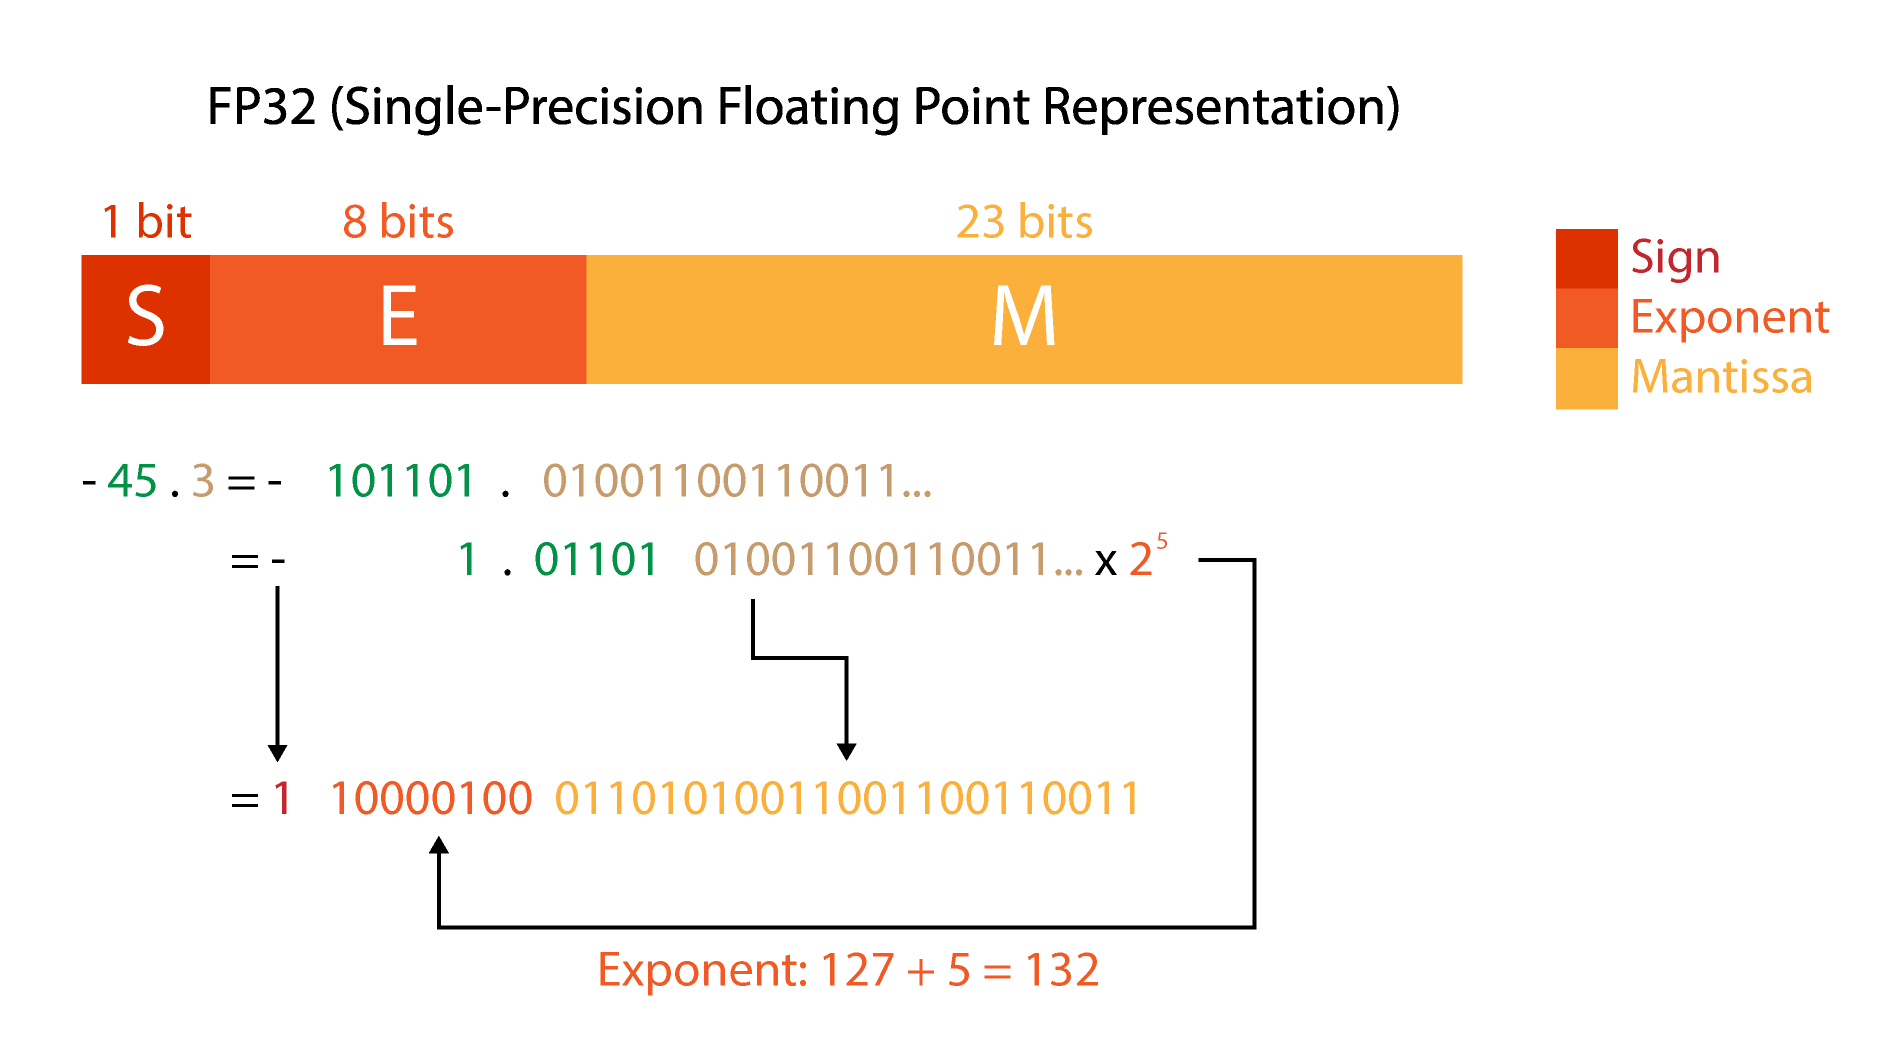
\includegraphics[width=.8\textwidth]{Figures/FP32.png}
	\caption[Single-precision float representation]{Example of the representation of a float in single-precision}
	\label{fig:FP32}
\end{figure}

% TODO CORRECT FIGURE

Referring to double precision floating-point representation means looking at 64-bit long memory representation, mapped as follows and as shown in \emph{Figure} \ref{fig:FP64}:
\begin{itemize}
  \item Sign bit: 1 bit
  \item Exponent: 11 bits
  \item Mantissa: 52 bits
  \item Exponent Bias: 127
\end{itemize}

% FP64 EXAMPLE
\begin{figure}[htbp]
	\centering
		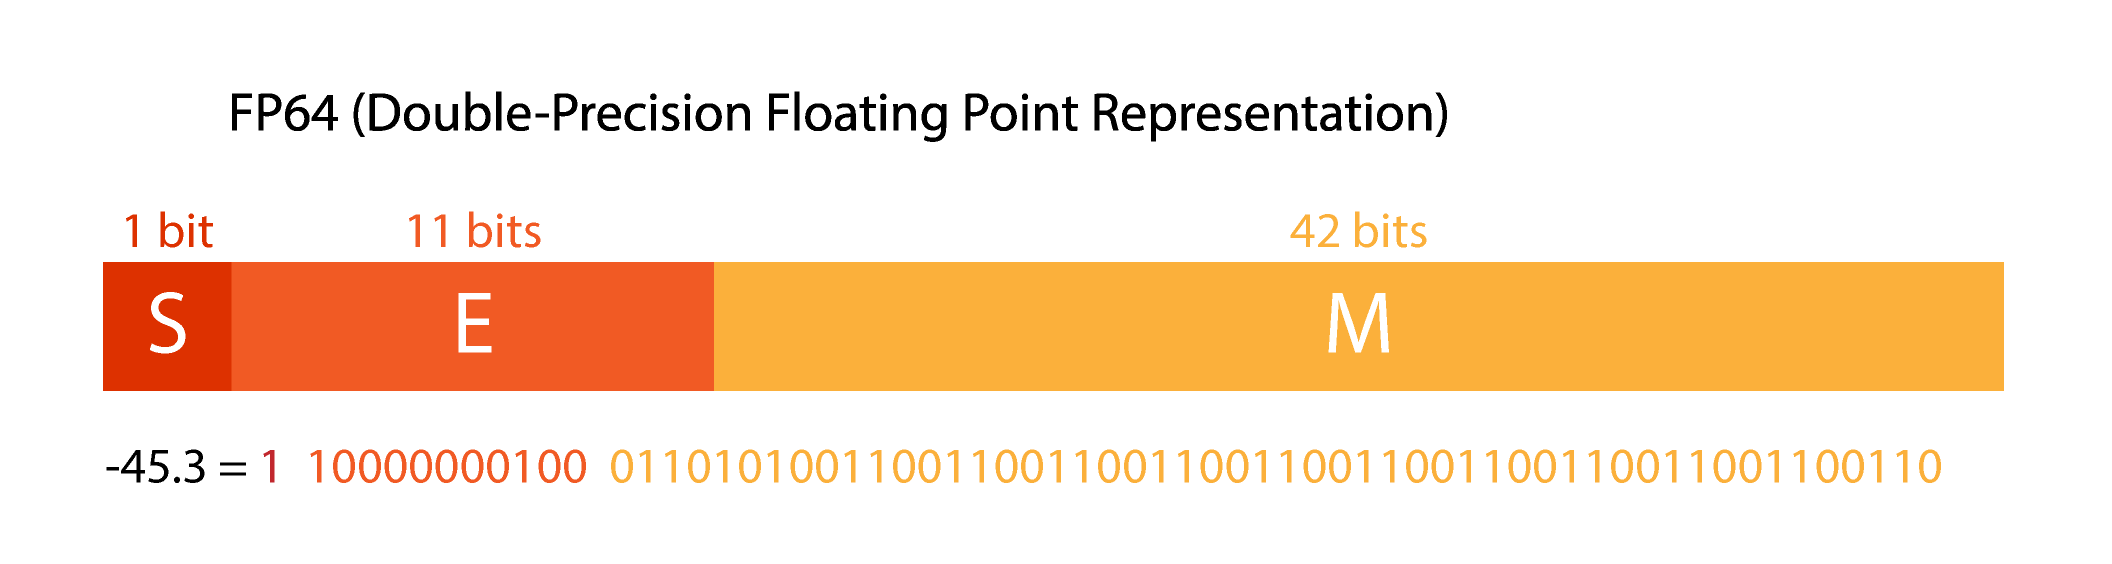
\includegraphics[width=.8\textwidth]{Figures/FP64.png}
	\caption[Double-precision float representation]{Example of the representation of a float in double-precision}
	\label{fig:FP64}
\end{figure}

% TODO CORRECT FIGURE

Along these representations, IEEE-754 introduces representations of special numbers. Positive and negative infinities are encoded with all 1s exponents and a fraction equal to zero. Zero is encoded with an all-0s exponent and fraction. Moreover, it adds methods to round floating-point numbers to positive or negative infinity, zero or to the nearest value.

%-----------------------------------
%	SUBSUBSECTION 2.1.1.3 - Fixed-Point Representation
%-----------------------------------
\subsubsection{Fixed-Point Representation}

Another way to look at the decimals is to fix the radix point to be at a certain place and keep it throughout all the computations and representations using this arithmetic. A fixed-point representation consists of three components:
\begin{enumerate}
  \item A sign indicator
  \item An integer corresponding to the total number of bits
  \item Another integer corresponding to the size of the fractional part
\end{enumerate}

Representing a number with this representation can be done by simply concatenating the base 2 representation of each side of the radix point. This means the integer part will be represented with positive powers of two ($2^0$,$2^1$,$2^2$,...) while the fractional part is represented with negative powers of two ($2^{-1}$, $2^{-2}$,...).

% FIXED POINT EXAMPLE
\begin{figure}[htbp]
	\centering
		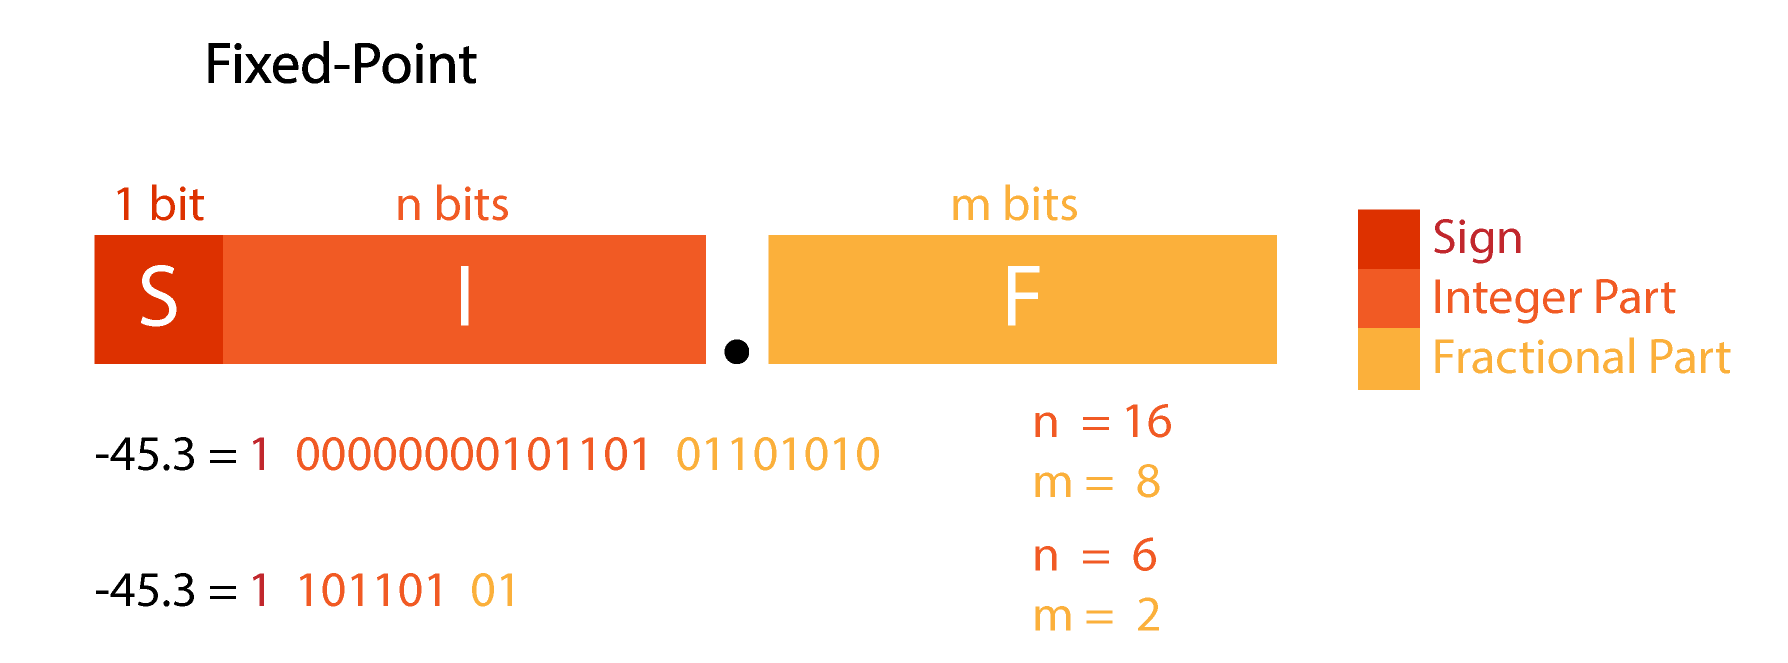
\includegraphics[width=.8\textwidth]{Figures/FixedPoint.png}
	\caption[Fixed-Point Representation]{Example of a float in fixed-point representation}
	\label{fig:FixedPoint}
\end{figure}

As shown in \emph{Figure} \ref{fig:FixedPoint}, several representations can depict the same decimal number. Finding the correct amount of bits to allocate to each side of the radix point is what will qualify the representation. Allocating fewer bits than needed may lead to overflow while allocating too much may increase quantisation errors.
Along with this new representation comes a whole new arithmetic. While this format can help tailor your needs in terms of variable types, it comes with an additional cost. The operations performed in this arithmetic are non-trivial as addition and multiplication are not associative and distributive anymore. This means the order of the operations will have an impact on the final result. Moreover, the round-off error underlying this representation is often non-trivial to grasp. However, those operations are low demanding in terms of computing power.

%-----------------------------------
%	SUBSECTION 2.1.2 - Performance Benchmarks
%-----------------------------------
\subsection{Metrics \& Performance benchmarks}

Floating-point representation (in either single or double precision) allows extreme precision at the cost of performance trade-offs (space or memory). On the other hand, fixed-point representation, even if it comes with a more complex arithmetic and insidious round-off errors, allows to tailor the type to your needs. Storing the values of the size and mass of planets in floating-point precision, would end up not using the majority of the range of values you selected while one could tailor a correct type in fixed-point representation.

The benchmarks in this field use several metrics in order to quantify and qualify the representations and their implementations.
\begin{itemize}
	\item \textbf{Size}: The size of a number in a given representation.
	\item \textbf{Energy cost}: The cost of operations in a given representation. \emph{The lower the better}.
	\item \textbf{Frequency}: The clock rate of a piece of hardware, or the quickness of pulses generation. \emph{The lower the better}.
	\item \textbf{Latency}: The access time of a piece of hardware to memory or external devices. \emph{The lower the better}.
	\item \textbf{Accuracy}: The precision enabled by a given representation. \emph{The higher the better}.
	\item \textbf{Memory Usage}: The memory needed to store both numbers and results of operations between them. \emph{The lower the better}.
	\item \textbf{Performance}: The overall time needed to complete a sequence of operations.
\end{itemize}

The operations performed in floating-point are expensive in terms of bandwidth, memory and energy consumption, which ultimately translate in to additional cost to perform an action. Horowitz's talk at ISSCC 2014 \cite{Horowitz2014} entitled \guille{Computing's Energy Problem (and what we can do about it)} provides an insight of the problems and challenges technology scaling has encountered in its development. Moore's law is getting outdated and a solution to the issue of permanently growing energy needs resides in \guille{the design of applications and hardware that are better matched to task and each other}. The numbers presented by M.Horrowitz have been reused by Professor William Dally (Standford University, NVidia Corporation) in his lecture on \guille{High-Performance Hardware for Machine Learning} \cite{Nips2015}. The \emph{Figure} \ref{fig:OpCosts} is extracted from this lecture and presents the energy and area costs different floating-point operations demand. Increasing precision on the used numbers increases the relative energy cost at the same time. An 8-bit addition costs 0.03 pJ whereas the same addition in 32-bit floating-point costs 0.9 pJ or 30 times more.

% COSTS OF OPERATIONS 2015-NIPS
\begin{figure}[htbp]
	\centering
		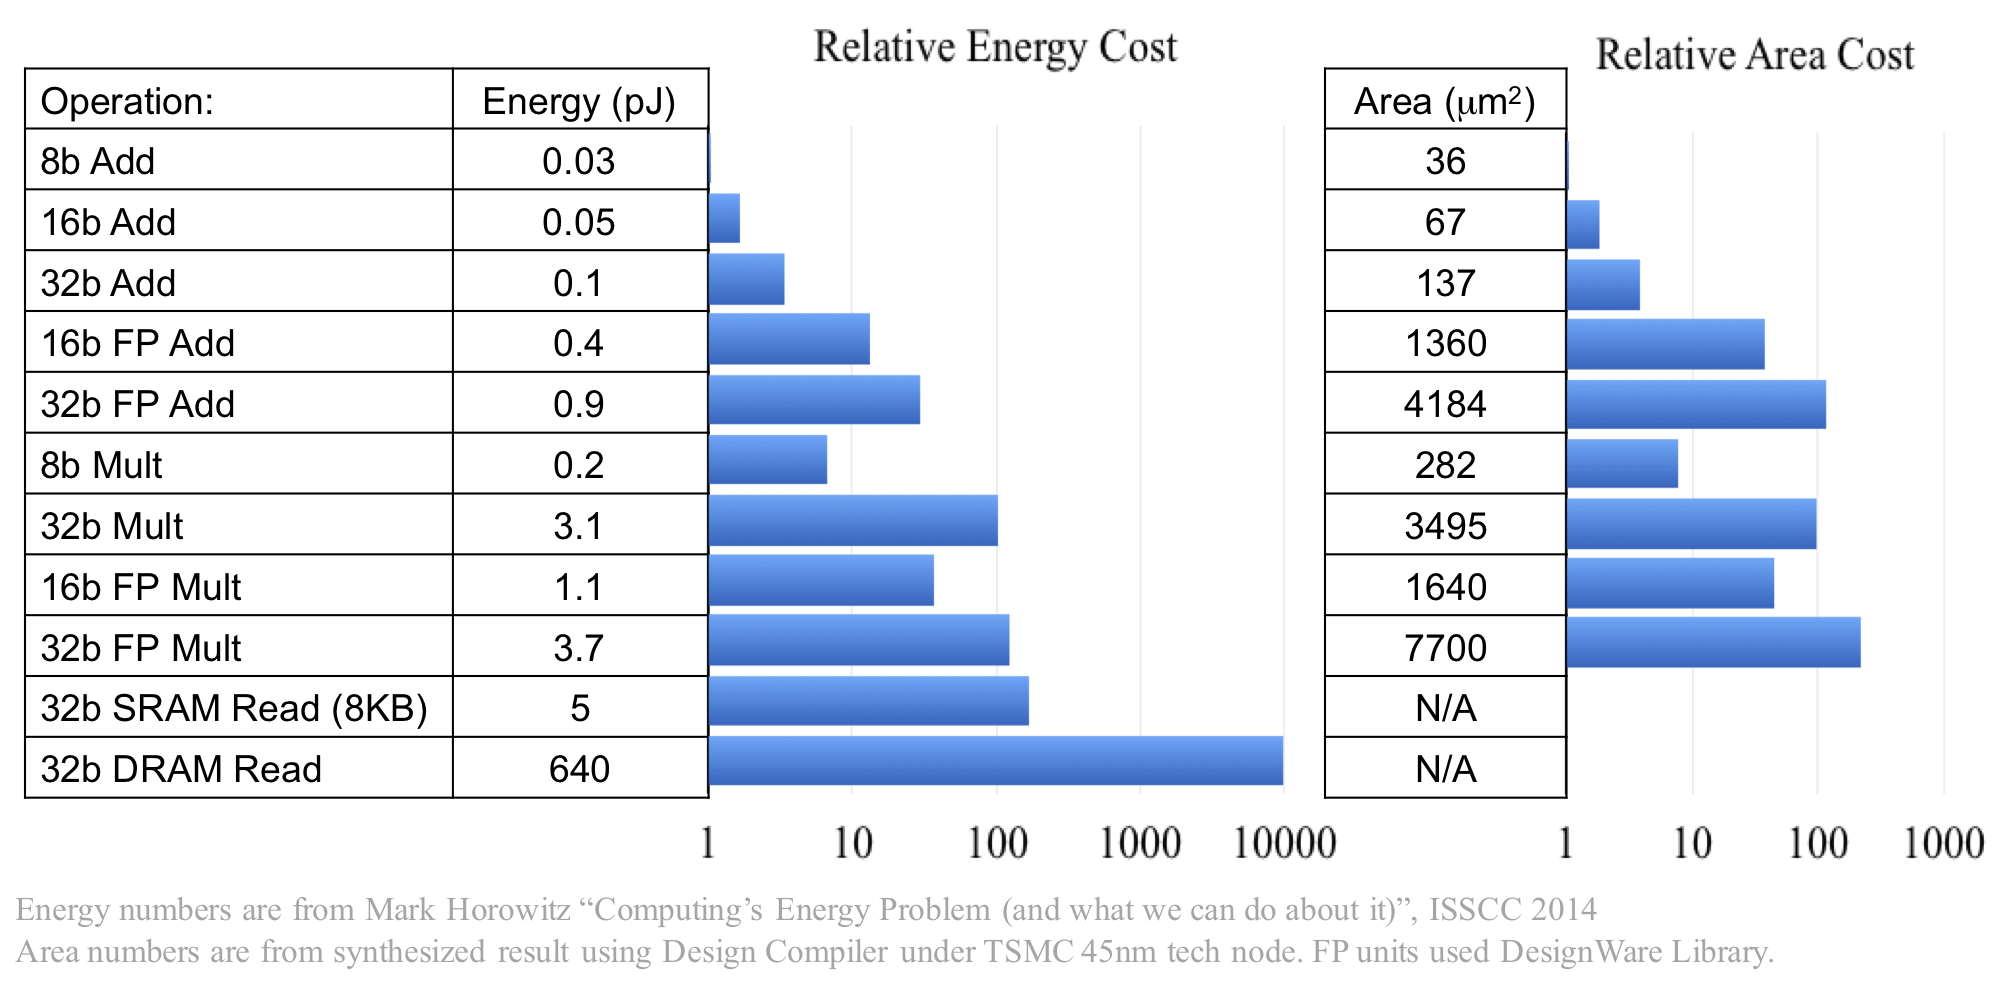
\includegraphics[width=\textwidth]{Figures/OpCosts.png}
	\caption[Operation costs]{Cost of operations in certain representations \cite{Nips2015,Horowitz2014}}
	\label{fig:OpCosts}
\end{figure}

The benefit of using a more optimised representation other the floating-point representation has been investigated as soon as in 2000 in \cite{Tong2000}. The authors present a way to reduce the energy consumption by minimising the bitwidth representation of the floating-point data. The data used to tailor the type representation is human-sensory data such as speech or video imagery. This kind of data is obtained at low precision (4 to 10 bits) but mapped into a full single-precision floating-point type. Using such optimisations, the authors manage to obtain a reduction of 66\% in multiplier energy per operation without sacrificing any accuracy.

Modifications of the representations can be embedded in the architecture. Xilinx, a manufacturer of state-of-the-art architecture, produced a white paper written by Finnerty et al. \cite{Xilinx2017} showing that their tools are able to handle fixed-point types and arithmetic and that the benefits are important:
\begin{itemize}
  \item Reduced power consumption
  \item Reduced use of resources (look-up tables, memory)
  \item Latency improvements
  \item Comparable performance and accuracy
\end{itemize}
The authors show the example of an FIR filter implementation in fixed-point representation from floating-point. The frequency is shown to be 16\% faster and the latency 7.5 times lower.

In conclusion, customising type in an environment where costs are translated in terms of energy consumption, memory or bandwidth usage, will always come out as an improvement. This redirects the issue to a need to guarantee little to no loss in accuracy.

%----------------------------------------------------------------------------------------
%	SECTION 2.2 - On Machine Learning
%----------------------------------------------------------------------------------------

\section{On Machine Learning}

Machine Learning is one of the most promising asset of the recent years since it has proven to be reliable when tackling complex issues. Those tasks can either be recognizing a street sign, a disease in a radiography or classifying a piece of text under a sentiment. Text-to-speech, speech-to-text, image classification, object detection, etc. Those are all thedomains machine learning is suited for. This section will provide insight on the basic functions machine learning uses, present neural network architectures and development frameworks.

%-----------------------------------------------
%	SUBSECTION 2.2.1 - Neurons and Neural Networks
%-----------------------------------------------

\subsection{Neural Networks}

 Machine learning has been extended to the use of neural networks. Karpathy et al. \cite{Karpathy2015} present the different structures in their lecture materials. The apparition of neural networks in machine learning comes from the analogy with the human brain and the way neurons work and communicate between each other. The analogy can be seen on \emph{Figure} \ref{fig:Neuron}.

% NEURON PRESENTATION
\begin{figure}[htbp]
	\centering
		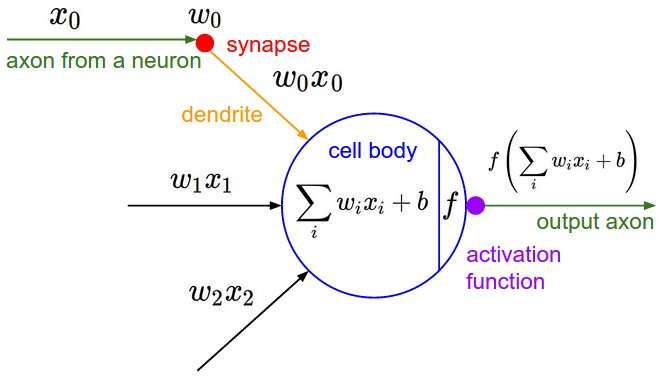
\includegraphics[width=8cm]{Figures/Neuron.png}
	\caption[Neuron Example]{Example of a neuron and its behavior in a neural network \cite{Karpathy2015}}
	\label{fig:Neuron}
\end{figure}

Each neuron receives several inputs from other previous neurons and performs an operation on all the received inputs to create the output that will go to its successors. A family of neurons that will obtain the outputs of the same neurons is called a \emph{layer}. A combination of \emph{layers} composes a \emph{neural network} as presented on \emph{Figure} \ref{fig:NN}.

% NEURAL NETWORK PRESENTATION
\begin{figure}[htbp]
	\centering
		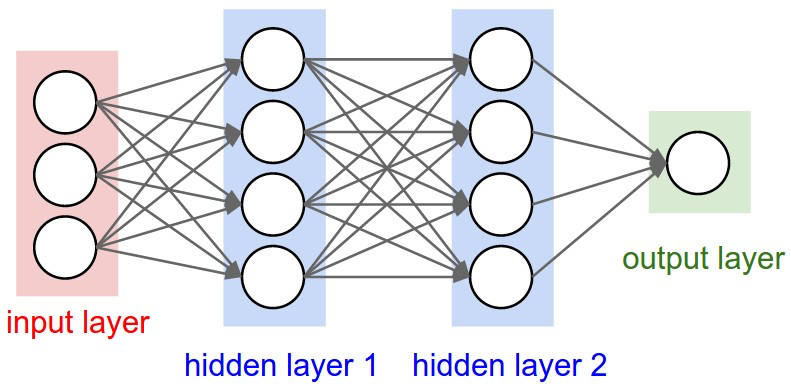
\includegraphics[width=8cm]{Figures/NN.png}
	\caption[Neural Network Example]{Example of a neural network architecture \cite{Karpathy2015}}
	\label{fig:NN}
\end{figure}

The neuron performs a simple dot product of all the inputs along with their weights, adds a bias to the sum and applies a given non-linear activation function. The weight will give importance to some of the inputs while hiding others. Throughout the training, some of the inputs will be shown to be more useful than others and their weight will be changed accordingly. The function used by the neuron (dot-product here) depends on the type of the layer the neuron is part of. The activation function models the \guille{firing rate of the neuron which [...] represents the frequency of the spikes along the axoms}. It is often a simple non-linear function that will help a network have an answer against non-linear problems. The XOR function for example can be learned by a network composed of as little as two layers. Several choices of non-linear functions can be made for your neurons:
\begin{itemize}
  \item Sigmoid function: $\sigma(x) = \frac{1}{(1+e^{-x})}$
  \item Tanh: $tanh(x) = 2\sigma(2x) - 1$
  \item Rectified Linear Unit (ReLU): $ f(x) = max(0,x) $
\end{itemize}

Neural networks perform the simple operations of reducing the inputs, adding a bias and passing it through a non-linear function. However, it is possible to set up several layers where the first one is called the \emph{input layer}, the last one the \emph{output layer} and all the layers in-between the \emph{hidden layers}. These layers go one after each other as shown in \emph{Figure} \ref{fig:NN}. While having hidden neurons is useful to better comprehend the data fed to the network, having too much of them can lead to overfitting, including noise and outliers into the pattern recognition.

% TODO ADD FIGURE FOR FORWARD PROP BACK PROP AND

A neural network \guille{learns} by tuning its parameters. The tuning occurs in two phases: a \emph{forward} and \emph{backward} propagation. The \emph{forward} propagation consists of running an instance through the whole network. The \emph{backward} propagation defines a cost function that will measure how good the neural network performs. This cost can be obtained for an instance and the corresponding output the network. The network adjusts the parameters by using partial differentiates on the cost function. This cost is determined by the \emph{loss function}. Another important piece of the workflow is the optimiser. If the \emph{loss function} can determine how wrong the predictions are, the optimiser is the actual function modifying the parameters. It can adopt different strategies, the most well-known being \emph{Gradient Descent}. The \guille{amount of change} the optimiser is able to add depends on a hyper-parameter, the \emph{learning rate}.

Neural networks perform well in machine learning, but the fields where the architecture is mostly used are image and speech recognition. An extension of neural networks is used when the data is known to be of a certain type. For example, if the data is known to be images, Convolutional Neural Networks (CNN) are the best choice as they are tailored with the goal of handling images. They are a special type of neural networks in the sense that they use 3D layers and transformations on images. This choice of 3D layers comes from the fact that images are usually encoded in three channels, RGB (Red, Green and Blue). CNNs can be used for image classification, object detection, image segmentation or speech recognition. We will focus on image recognition here as this field provides well-known metrics and network layouts due to the popularity of the ImageNet Project for example \cite{ImageNet2009}. This popularity has attracted literature focus and allows comparisons and benchmarks to be made.

% NEURAL NETWORK PRESENTATION
\begin{figure}[htbp]
	\centering
		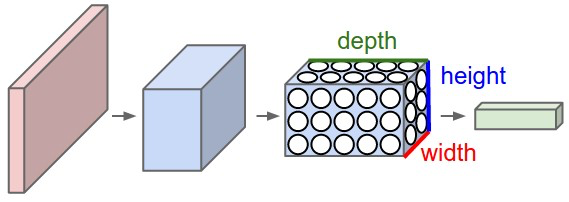
\includegraphics[width=8cm]{Figures/CNN.png}
	\caption[Convolutional Neural Network Example]{Example of a convolutional neural network architecture \cite{Karpathy2015}}
	\label{fig:CNN}
\end{figure}

Several layers are used and allow to perform different operations on images. The most used and well-known are the following:
\begin{itemize}
  \item Convolution   (CONV): Connects small regions of the input image through a filter. \emph{This layer helps extracting features such as edges or shapes.}
  \item Activation     (ACT): Apply an activation function (such as $max(0,x)$). \emph{This layer brings non-linearity into place.}
  \item Pooling       (POOL): Downsampling operation through a filter. \emph{This layer replaces a region of the image with the max or average value. It helps reducing noise.}
  \item Fully-Connected (FC): Computation of the class scores. \emph{This layer consists of a reduce operation and allows to compute the class scores.}
\end{itemize}

Layers take as input a set of data, known as a \emph{Feature Map} and output a new set of feature maps with higher-level semantics. Those layers then compose a CNN architecture and can be trained on a bank of images to adjust the different bias and weights for each layers and their corresponding neurons. Finally, once the network is trained, it can deduce the class of a given image. Those two steps are called \emph{Training} and \emph{Inference}, the training will work on a set of annotated data samples to create a model \guille{which semantics extrapolate outside the training set, [with a] \emph{modelling power}} \cite{Abdelouahab2018}. Once this step is completed, the \emph{Inference} phase can start and the network will have to classify new data instances. The training phase is extremely consuming in terms of time, energy and hardware resources. However, it only needs to be performed once. On the other hand, the inference has to be run each time a new instance is provided to the system. Therefore, if literature focus on accelerating both phases, an emphasis is put on inference as it will be needed to embark trained networks in lighter architectures.

%-------------------------------------------------
%	SUBSECTION 2.2.2 - Tools for Classification
%-------------------------------------------------

\subsection{Tools for Classification}

%-----------------------------------------------
%	SUBSUBSECTION 2.2.2.1 - Network Architectures
%-----------------------------------------------

\subsubsection{Network Architectures}

While there exists a wide range of applications for neural networks and machine learning in general, the field of image classification is the most suitable to benchmarking. Literature presents a wide and evergrowing number of neural networks, often backed up by reknowned companies. Historically, Yann Le Cun et al. \cite{LeCun1998} presented the first version of a CNN tailored to a specific task: recognizing handwritten digits. By the same occasion, they created the MNIST (Modified National Institute of Standards and Technology) dataset to benchmark their network architecture. All CNN architectures are composed of two main phases:
\begin{itemize}
  \item \emph{Feature Extraction}: This phase consists of an extraction of features by downsampling the image through several filter layers (convolutions, pooling but also batch normalisation and dropout).
  \item \emph{Classification}: This phase consists of flattening the output of the first phase and running it through several linear layers with varying number of neurons. The final linear layer will always have a number of neurons equal to the number of classes in the classification challenge.
\end{itemize}

The following figures are taken from Raimi Karim work for \emph{Towards Data Science} in \cite{Karim2020}.

Le Cun et al. \cite{LeCun1998} architecture chose to tackle the two phases by designing a neural network architecture called \emph{LeNet}. This architecture represents the feature extraction phase by using a succession of two $5 \times 5$ convolutions and $2 \times 2$ average pooling layers. Then, three linear layers (fully connected) perform the classification. Their respective size are 120, 84 and 10 (the number of classes in MNIST \cite{LeCun2010} case which it was designed for). The activation function used is hyperbolic tangent. This whole architecture is displayed on \emph{Figure} \ref{fig:LeNet-5} representing the version \emph{LeNet-5}.

% LeNet-5 PRESENTATION
\begin{figure}[htbp]
	\centering
		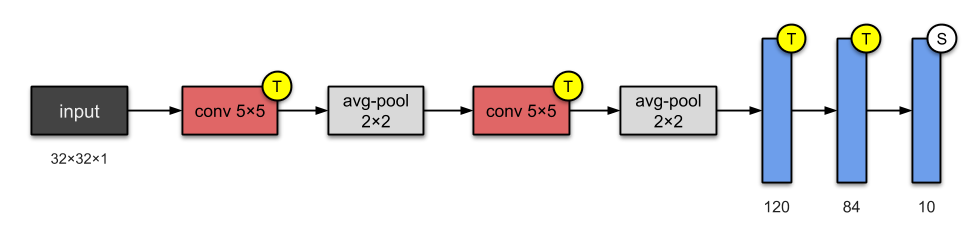
\includegraphics[width=10cm]{Figures/LeNet-5.png}
	\caption[LeNet-5]{Architecture of LeNet-5 as taken from \cite{LeCun1998}}
	\label{fig:LeNet-5}
\end{figure}

Krizhevsky et al. present \emph{AlexNet} \cite{Krizhevsky2012} in 2012, 14 years later, as the succesor of \emph{LeNet}. \emph{AlexNet} consists of deeper and wider version of \emph{LeNet}. There are now five convolution layers (of respective filter size $11 \times 11$, $5 \times 5$ and $3 \times 3$ for the remaining). Maximum pooling is used instead of average and it is the first time the ReLU function is used as an activation function ($max(0,x)$ as a reminder). The three final layers are now sized as 4096, 4096 and 1000 (the number of classes of the ImageNet \cite{ImageNet2009} dataset). This whole architecture is displayed on \emph{Figure} \ref{fig:AlexNet}.

% AlexNet PRESENTATION
\begin{figure}[htbp]
	\centering
		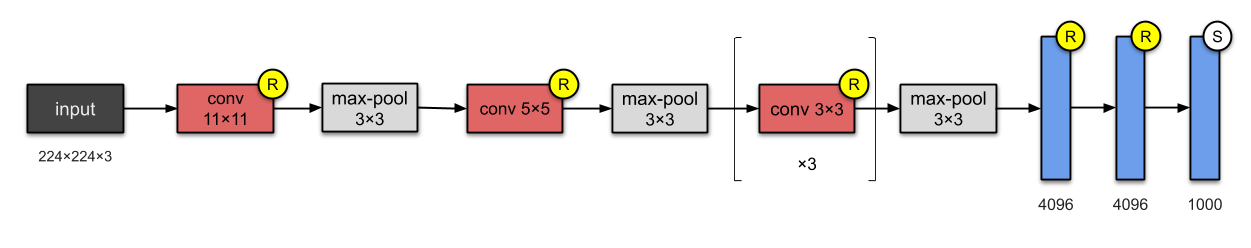
\includegraphics[width=12cm]{Figures/AlexNet.png}
	\caption[AlexNet]{Architecture of AlexNet as taken from \cite{Krizhevsky2012}}
	\label{fig:AlexNet}
\end{figure}


Using the same idea that Krizhevsky et al. \cite{Krizhevsky2012} had in mind when designing \emph{AlexNet} in 2014, Simonyan et al. took it a step further when designing \emph{VGGNet} \cite{Simonyan2014}. The VGG net comes with different versions (11, 13, 16 and 19) corresponding to the number of convolutions and fully-connected layers. Using only $3 \times 3$ convolution filters and the same size of linear layers, VGG-16 performed very well on ImageNet \cite{ImageNet2009}. Its architecture is displayed on \emph{Figure} \ref{fig:VGG-16}. One of the downside of this very-deep neural network is that it holds an enormous amount of parameters taking memory space. VGG-16 for example takes about 500MB of memory.

% VGG-16 PRESENTATION
\begin{figure}[htbp]
	\centering
		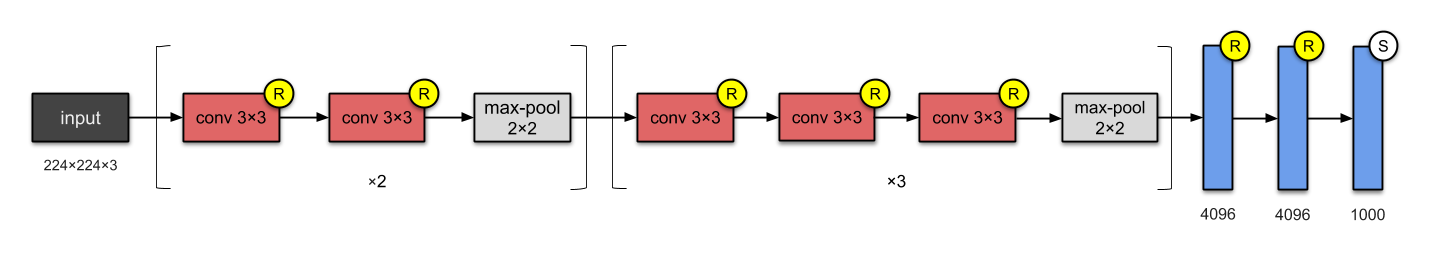
\includegraphics[width=14cm]{Figures/VGG-16.png}
	\caption[VGG-16]{Architecture of VGG-16 as taken from \cite{Simonyan2014}}
	\label{fig:VGG-16}
\end{figure}

From now on, extending the layer size and network depth does not seem to give better results. Reknowned companies are now enrolling in the battle to the best accuracy on the ImageNet dataset \cite{ImageNet2009} and Microsoft presents its \emph{ResNet} \cite{He2015} in the 2015 competition. \emph{ResNet} uses a method to add a way to skip some connections. During the training of a network, all weights receive an update proportional to the gradient. If this gradient is very small, the change in weight can be minimal and the network can stop its training. Microsoft Research used those skipping connections to conserve the signal and mitigate data loss. In other words, \emph{ResNet} breaks a deep neural network into smaller networks connected through skip or shortcut connections. Its architecture is displayed on \emph{Figure} \ref{fig:ResNet-50}.

% ResNet-50 PRESENTATION
\begin{figure}[htbp]
	\centering
		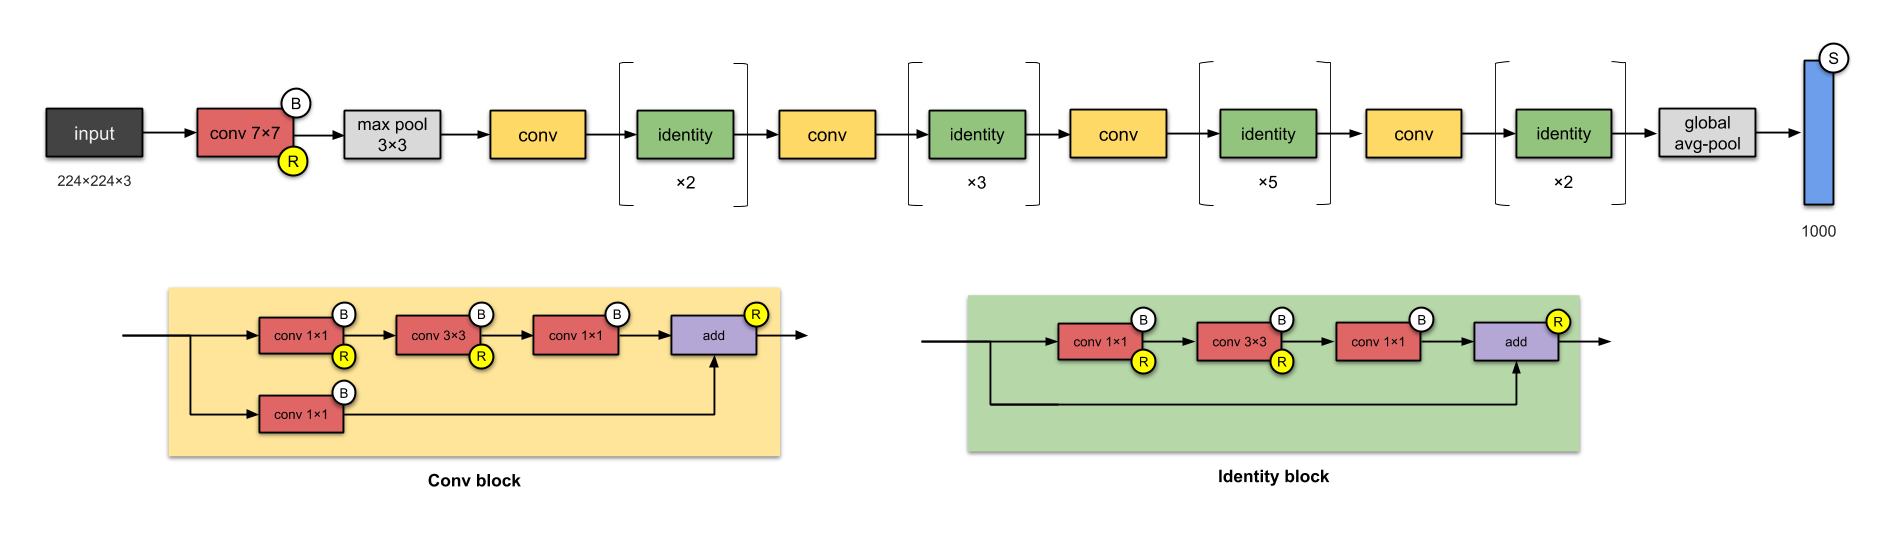
\includegraphics[width=15cm]{Figures/ResNet-50.png}
	\caption[ResNet-50]{Architecture of ResNet-50 as taken from \cite{He2015}}
	\label{fig:ResNet-50}
\end{figure}

Google came into place by proposing the \emph{MobileNet} \cite{Howard2017} architecture. This architecture, as its name shows, aims at being embarked in many mobile or light hardware architectures. Its emphasis is put on the size of the network and should allow the developer to tailor it to the needs of his aimed hardware architecture. The number of parameters is reduced by using a \guille{\emph{separable depthwise convolution}} that separates the usual $3 \times 3$ convolution into two parts. The first one applies the filter on the inputs and the second (a $1 \times 1$ filter called \guille{\emph{pointwise convolution}}) combine the outputs. Overall, this technique allows to reduce the number of parameters and operations while keeping state-of-the-art.

% % MobileNet PRESENTATION
% \begin{figure}[htbp]
% 	\centering
% 		\includegraphics[width=8cm]{Figures/MobileNet.png}
% 	\caption[MobileNet]{Architecture of MobileNet as taken from \cite{He2015}}
% 	\label{fig:MobileNet}
% \end{figure}

Many other networks exist and are still being developed actively. New techniques (e.g. batch normalisation \cite{Ioffe2015}) are getting incorporated in state-of-the-art architectures to get an even better result out of them. This list is in no way exhaustive but presents the milestones and wishes to translate the mindset operating in the machine learning community.

\emph{Table} \ref{tab:CNNTable} summarizes the different network architectures. It provides both the network\'s name, year, paper it has been extracted from as well as its number of parameters. Moreover, the \emph{top-1} accuracy of the network on the ImageNet \cite{ImageNet2009} dataset is provided. We can see, as said earlier, that extending the network\'s number of parameters has been the focus of state-of-the-art architectures until 2014. After that, the focus has shifted to change the neural networks mechanics more deeply. The \emph{ResNet} for example brings a new method to keep \emph{residuals} or \emph{MobileNet} that brings specific convolutions, \emph{depth- and point-wise} in order to reduce the overall number of parameters.

\begin{table}[!]
  \centering
  \resizebox{\textwidth}{!}{
  \begin{tabular}{ | c | c | c | c | c | }
    \hline
    \textbf{Name}          & \textbf{Year} &    \textbf{Paper}     & \textbf{Number of Parameters} & \textbf{Top-1 Accuracy} \\
    \hline
    \textbf{LeNet}         &     1998      &  \cite{LeCun1998}     &         0.6 M                 &           X             \\
    \hline
    \textbf{AlexNet}       &     2012      & \cite{Krizhevsky2012} &          60 M                 &         63.3\%          \\
    \hline
    \textbf{VGGNet (16)}   &     2014      & \cite{Simonyan2014}   &         138 M                 &         74.4\%          \\
    \hline
    \textbf{ResNet (50)}   &     2015      & \cite{He2015}         &          26 M                 &         81.2\%          \\
    \hline
    \textbf{MobileNet}     &     2017      & \cite{Howard2017}     &         4.2 M                 &         72.56\%         \\
    \hline
  \end{tabular}
  }
\caption[CNNTable]{Convolutional Neural Network Architectures}
\label{tab:CNNTable}
\end{table}

%----------------------------------
%	SUBSUBSECTION 2.2.2.2 - Datasets
%----------------------------------

\subsubsection{Datasets}

The architectures presented earlier are well-known and are still getting better with version iterations and the discovery of new techniques (batch normalisation, depth-wise convolution, residuals, etc.). On the other side, datasets have evolved to present each time a new and harder challenge for different architectures to perform on. Well-known datasets consist of the following:
\begin{itemize}
  \item \emph{MNIST} is the historical dataset, considered as the machine learning version of a classic \guille{\emph{hello world}}. It was implemented along with the \emph{LeNet} architecture and has been the default first dataset to train a network architecture on ever since. Several extensions to this dataset have been created since the dataset is juged to be \guille{too easy} to be a challenge to modern neuron architectures. Very simple CNN can achieve less than 3\% error on this dataset. Several drop-in replacements have been developed such as \emph{Fashion-MNIST} \cite{Xiao2017} - set up by Zalando with simple images of garnments -, \emph{Kuzushiji-MNIST} \cite{Clanuwat2018} - three versions on the recognition of Japanese characters - or even \emph{MNIST-MIX} \cite{Jiang2020} - a mix of handwritten digits from different languages -. All the instances of the MNIST dataset and its variations are images with only one channel (grey levels) and sized 28 pixels by 28 pixels. Those images are labelled in 10 different classes (digits from 0 to 9).

  % MNIST PRESENTATION
  \begin{figure}[htbp]
  	\centering
  		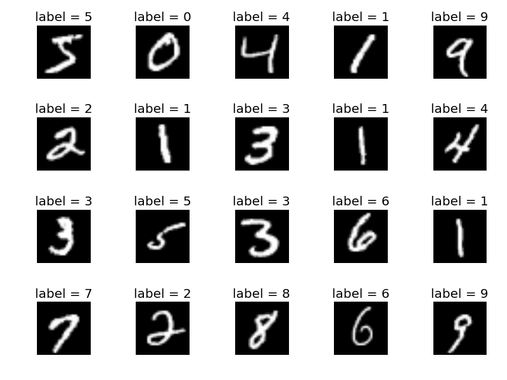
\includegraphics[width=8cm]{Figures/MNIST.png}
  	\caption[MNIST]{Instances extracted from the MNIST dataset}
  	\label{fig:MNIST}
  \end{figure}

  \item \emph{CIFAR-10} are labelled subset from the \emph{Tiny Images} dataset \cite{Krizhevsky2009}. It has been created in 2009 as collected and labeled automatically, supervised by three researchers from the MIT. This dataset is composed of tiny ($32 \times 32$) colored (3 channels) images of ten different classes: airplane, automobile, bird, cat, deer, dog, frog, horse, ship and truck. Instances taken from this dataset can be seen on \emph{Figure} \ref{fig:CIFAR-10} A more complicated dataset has been created in the same way. It is called \emph{CIFAR-100}, and as its name might suggest, contains a hundred different classes.

  % CIFAR-10 PRESENTATION
  \begin{figure}[htbp]
  	\centering
  		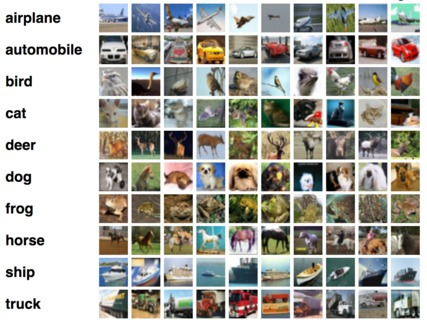
\includegraphics[width=8cm]{Figures/CIFAR-10.jpg}
  	\caption[CIFAR-10]{Instances extracted from the CIFAR-10 dataset}
  	\label{fig:CIFAR-10}
  \end{figure}

  \item With a growing emphasis put on autonomous vehicles, datasets have been developed accordingly. The two most well-known datasets covering this area are \emph{SVHN} (Street View House Numbers) \cite{Netzer2011} and \emph{GTSRB} (German Traffic Sign Recognition Benchmark) \cite{Stallkamp2012}. These two datasets have colored images of variable dimensions. \emph{SVHN} is an extension of \emph{MNIST} in the sense that it is a combination of different digits that the network will have to recognize. On the other hand, \emph{GTSRB} has been used in a 2012 competition and is useful to prototype self-driving components. \emph{GTSRB} contains 43 different classes of colored images and an instance of each of them can be seen on \emph{Figure} \ref{fig:GTSRB}.

  % % SVHN PRESENTATION
  % \begin{figure}[htbp]
  % 	\centering
  % 		\includegraphics[width=8cm]{Figures/SVHN.png}
  % 	\caption[SVHN]{Instances extracted from the SVHN dataset}
  % 	\label{fig:SVHN}
  % \end{figure}

  % GTSRB PRESENTATION
  \begin{figure}[htbp]
  	\centering
  		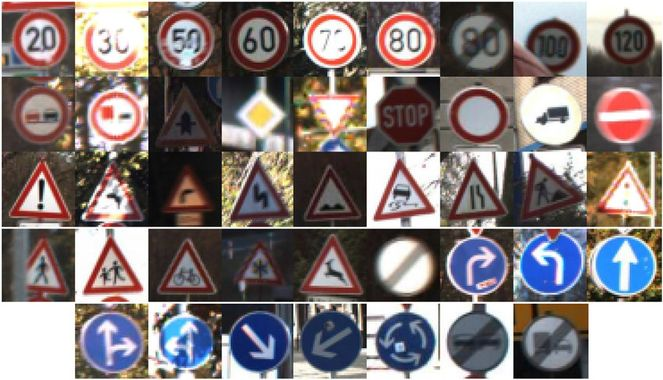
\includegraphics[width=8cm]{Figures/GTSRB.jpeg}
  	\caption[GTSRB]{Instances extracted from the GTSRB dataset}
  	\label{fig:GTSRB}
  \end{figure}

  \item Finally, \emph{ImageNet} \cite{ImageNet2009} is one of the largest dataset developed. It has been put up by a team from the Princeton University and is the centre of a challenge each year where state-of-the-art architectures confront themselves to get the best accuracy possible. The challenge is named the ImageNet Large Scale Visual Recognition Challenge (ILSVRC). Every year, contesters try to get the best possible accuracy out of the network they propose. The images contained in the dataset are $224 \times 224$ colored images split in 20,000 classes. The dataset contains more than 14 million images and has become the benchmark to determine the accuracy and robustness of state-of-the-art architectures.

  % IMAGENET PRESENTATION
  \begin{figure}[htbp]
  	\centering
  		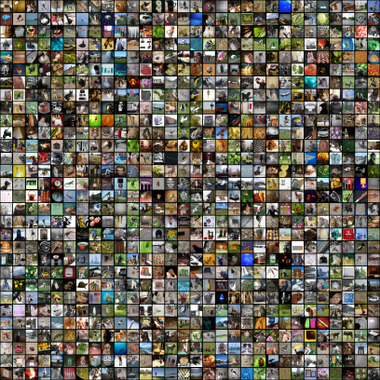
\includegraphics[width=8cm]{Figures/ImageNet.png}
  	\caption[ImageNet]{Instances extracted from the ImageNet dataset}
  	\label{fig:ImageNet}
  \end{figure}

\end{itemize}

% TODO: INCLUDE Table simplifying the different datasets

\begin{table}[!]
  \centering
  \resizebox{\textwidth}{!}{
  \begin{tabular}{ | c | c | c | c | c | c | c | }
    \hline
    \textbf{Name}            & \textbf{Year} &    \textbf{Paper}     & \textbf{Channels} & \textbf{Image Size} & \textbf{Instances}  & \textbf{Number of Classes} \\
    \hline
    \textbf{MNIST}           &     1998      &  \cite{LeCun1998}     &  1 (Grayscale)    &   $28 \times 28$    &  60,000 / 10,000    &    10     \\
    \hline
    \textbf{FashionMNIST}    &     2017      & \cite{Xiao2017}       &  1 (Grayscale)    &   $28 \times 28$    &  50,000 / 10,000    &    10     \\
    \hline
    \textbf{Kuzushiji-MNIST} &     2018      & \cite{Clanuwat2018}   &  1 (Grayscale)    &   $28 \times 28$    &  60,000 / 10,000    &    10     \\
    \hline
    \textbf{MNIST-MIX}       &     2020      & \cite{Jiang2020}      &  1 (Grayscale)    &   $28 \times 28$    & 397,440 / 99,360    &   100     \\
    \hline
    \textbf{CIFAR-10}        &     2009      & \cite{Krizhevsky2009} &  3 (RGB)          &   $32 \times 32$    &  50,000 / 10,000    &    10     \\
    \hline
    \textbf{CIFAR-100}       &     2009      & \cite{Krizhevsky2009} &  3 (RGB)          &   $32 \times 32$    &  50,000 / 10,000    &   100     \\
    \hline
    \textbf{SVHN}            &     2011      & \cite{Netzer2011}     &  3 (RGB)          &   $32 \times 32$    &  73,260 / 26,000    &    10     \\
    \hline
    \textbf{GTSRB}           &     2012      & \cite{Stallkamp2012}  &  3 (RGB)          &   $15 \times 15$ to $250 \times 250$      &    50,000 / 10,000   &    43     \\
    \hline
    \textbf{ImageNet}        &     2009      & \cite{ImageNet2009}   &  3 (RGB)          &  $224 \times 224$   &   14M / 50,000      &  1000     \\
    \hline
  \end{tabular}
  }
\caption[DatasetTable]{Datasets}
\label{tab:DatasetTable}
\end{table}

%-----------------------------------------------------
%	SUBSUBSECTION 2.2.2.3 - Development Frameworks
%-----------------------------------------------------

\subsubsection{Development Frameworks}

As research in the field of machine learning keeps growing and attracting more and more focus, many different development frameworks emerged to propose a high-level API and environment to experimental needs. Major industrial actors used this opportunity to present their own development API. Most of them have been under development for nearly a decade and still continue to attract a growing audience.

\begin{itemize}
  \item \emph{Tensorflow} has been the initiative of Google in 2011 and its source code has been opened in 2015. It is, to this day, the most used development framework in the field of machine learning. Its API is designed for Python and C++. However, due to increasing attention, numerous bindings to other languages have been created (Java, C\#, Haskell, etc.). Tensorflow set the milestones for AI frameworks by implementing production-ready resource distribution to deploy one's network to anyy architecture (CPU, GPU or a cluster). It also implements the idea of a \emph{tensor}, a ditributed array.
  \item Microsoft launched in 2015 its \emph{Cognitive Toolkit (CNTK)} written in C++ that aims at the same objectives as \emph{Tensorflow}: easy network creation through a high-level API and simplified deployment to a variety of architectures.
  \item The first version of \emph{Caffe (Convolutional Architecture for Fast Feature Embedding)} was developed in the University of Berkeley in 2014. In 2017, Facebook used \emph{Caffe} in an extended version called \emph{Caffe2} and as of May 2018, \emph{Caffe2} is officially merged in the \emph{PyTorch} project.
  \emph{Torch} is a Lua-based framework that was created in 2002. It is not in active development anymore since 2018 but \emph{PyTorch}, a Python implementation of the same underlying logic is in active development with a specific focus on the research community. \emph{Pytorch} aims at rapid prototyping and flexible architectures.
\end{itemize}

In the end, choosing a framework depends on one's objectives and knowledge of the language used. Benchmarks are getting released with, for example, Luo et al. \cite{Luo2020} that present a mobile implementation of several network architectures (\emph{ResNet, Inception, DenseNet, etc.}) implemented in \emph{TensorFlow Lite, Caffe2 and PyTorch Mobile}. The benchmark the authors propose is named \emph{AIoTBench} and focuses on computer vision. Few other initiatives have been published. The choice is purely personal for now.

% TODO: INCLUDE Table comparing the different development frameworks

%----------------------------------------------------------------------------------------
%	SECTION 2.3 - Hardware Architecture
%----------------------------------------------------------------------------------------

\section{On Hardware Architecture}

Moore's law \cite{Moore2006} predicted the evolution of hardware capacities in years to come when defined in 1965. It is an empirical relationship and in no means a physical or natural law but has shown to be exact for the thirty years following its creation. The Moore's law, when announced in 1965 said that \guille{the number of components per integrated circuit would double every year}. This law held for a decade and was then revised to \guille{doubling every two years} for the next decade. This law has been an industry guideline and helped produce long term business plans. However, the law is slowly coming to an end and has been shown to not fulfill the prophecy anymore due to physical limitations such as thermal restrictions. New architectures will have to take the lead as more computational power is still needed for the years to come. What are the new ways and architectures to increase performance even more?

%-----------------------------------
%	SUBSECTION 2.3.1 - GPU
%-----------------------------------

\subsection{GPU}

One solution to enable hardware acceleration is to parallelise computationally expensive tasks. GPUs (\emph{Graphics Processing Units}) are specialised electronic circuits that can handle computationally demanding tasks such as 3D rendering, video encoding and decoding or any action that can be massively parallelised (cryptocurrency digging, matrix computations or brute-force cracking). Few companies actually conceive and sell such systems. The most famous are NVidia, AMD and Intel and some smaller fabless - conceive the circuit but integrally subcontract the production -  companies such as Qualcomm or ARM. Other manufacturing companies such as ASUS or MSI will then integrate those circuits into products and calibrate them along with a cooling system that can make it enhance its base abilities.

Along with GPUs come their proper Software Development Kit (SDK) in order for developers to use their tools. NVidia invested heavily in CUDA (\emph{Compute Unified Device Architecture}) \cite{CUDA} and its aim is to reproduce a C syntax and environment for GPUs. AMD and Intel provide open-source SDK that tools then built upon.

GPUs allow computers to delegate expensive tasks (3D rendering for example) from the CPU to them. The GPUs can be either integrated or external. They require less knowledge than FPGAs but provide a more static architecture that will limit tuning opportunities. Mixed-precision mindset will not reach its full potential with this architecture but will still manage to increase the performance of different operations and tasks.

GPU provide an easy access to parallelisation and allow researchers of different fields to experiment with different precisions and parallelisation. One field that benefits a lot from it is the field of physics and applied simulations. Inherently, mathematics benefit a lot from reduced precisions in terms of computation times and resource utilisation to perform clasic operations such as matrix factorisation. Next are some examples of GPU application in the world of mixed-precision along with the hardware used.

\begin{itemize}
  \item \emph{Mathematics:} Haidar et al. \cite{Haidar2018} present a mixed-precision method to factorise a matrix into two triangular matrices. In order to perform their experiments, they use two 10-cores \emph{Intel Xeon e5-2650 v3} CPUs and one \emph{NVidia V100 PCLe} GPU.
  \item \emph{Mechanical Engineering:} Goddeke et al. \cite{Goddeke2007} present a survey paper on mixed-precision applied to \emph{Finite Element Simulations}, a widely used method in physics simulations that often require extensive computational resources. In their experiments, they use an \emph{AMD Athlon64 X2 4400} CPU and an \emph{NVidia GeForce 7800 GTX} GPU.
  \item \emph{Geosimulation:} Ichimura et al. \cite{Ichimura2018} present a mixed-precision earthquake simulator with an IA designed to help the solver converge. They use several super-computers such as the \emph{Summit} comprising two \emph{IBM Power9} processors and six \emph{NVidia Volta V100 accelerators}.
  \item \emph{Nuclear physics:} Clark et al. \cite{Clark2010} use mixed-precision in their work on simulating the quarks\' interactions in a nucleon. They use an \emph{NVidia GeForce GTX 280} GPU.
\end{itemize}

GPUs represent a fair part of the marketshare due to their various usages. They often come as a cheap and easy access to parallelisation since they have a wide and diverse community with ready-to-go frameworks and implementations.

%-----------------------------------
%	SUBSECTION 2.3.2 - FPGA
%-----------------------------------

\subsection{FPGA}

On the other hand, the 1990's have seen the birth of a new type of architecture: reconfigurable hardware. They allow to create application-specific hardware and are mixed-precision by default. Xilinx, one of the most famous FPGA manufacturer describes them as consisting of \guille{up to two million logic cells that can be configured to implement a variety of software algorithms} \cite{Xilinx2017}. Those logic cells can be dynamically reconfigured and this is the strength of this architecture.

Modern FPGAs contain components that are specialised for specific functions as well as more general purpose configurable logic. The combination of specific components with the configurable logic has allowed for architectures that consume less power and perform more efficiently.
\begin{itemize}
  \item \emph{Configurable Logic Block (CLB):} A \emph{CLB} is the most basic FPGA component which provide both logic and storage functionalities. It can be anything like a transistor, NAND gate, multiplexor or any combination of these. It often comes with a \emph{Look-Up Table (LUT)} to perform logic operations and a \emph{Flip-Flop (FF)} acting as a register for the results of the \emph{LUT}.
  \item \emph{Digital Signal Processing (DSP) Block:} A \emph{DSP block} is a specialised component of an FPGA that is designed to carry out \emph{digital signal processing} functions such as filtering or multiplying. It is designed to be much more efficient than if it was made with several \emph{CLBs}.
  \item \emph{Transceiver:} A \emph{trans-ceiver} is made to \emph{trans}-mit and re-\emph{ceive} serial data (individual bits) to and from the FPGA at extremely high rates. It also checks for erroneous data in the transmission. Having a dedicated component made it both quicker and easier to communicate with the FPGA.
  \item \emph{Block Random Access Memory (BRAM):} A \emph{BRAM} is the dedicated memory on the chip. This type of block can be divided or cascaded to make smaller or larger memory chunks available.
  \item \emph{Input/Output (I/O) Block}: The \emph{I/O block} operates, as its name gives out, as a component through which data transfers in and out of the FPGA. They are similar to \emph{transceivers} but are more flexible in functionality while operating at slower speed.
\end{itemize}

Along with those base components come many high-end more interesting components that can help develop the hardware to be tightly linked to the application one has in mind. As stated by \cite{Goddeke2007}, FPGAs have native mixed-precision processors and \guille{there is no need to utilise the same number format throughout the algorithm, or even the same operation}. Moreover, the freedom in the number representation can lead to alternative feasible number representations, such as a logarithmic one.

FPGAs can help prototyping chips and perform system validation, including pre-silicon validation, post-silicon validation and firmware development. Manufacturers can therefore validate their design before the chip is produced in factory. The end product can be an ASIC for example, an extremely powerful computing unit that is tailored to one function and one function only. Even though FPGAs are slower than ASICs and consume more power, their inherent ability to be reconfigurable makes them interesting in certain applications. Microsoft uses FPGAs to speed up Bing searches and still be able to change the search algorithm if needed. The efficiency versus flexibility can be seen on \emph{Figure} \ref{fig:EfficiencyVSFlexibility}.

% FPGA/ASIC comparison
\begin{figure}[htbp]
	\centering
		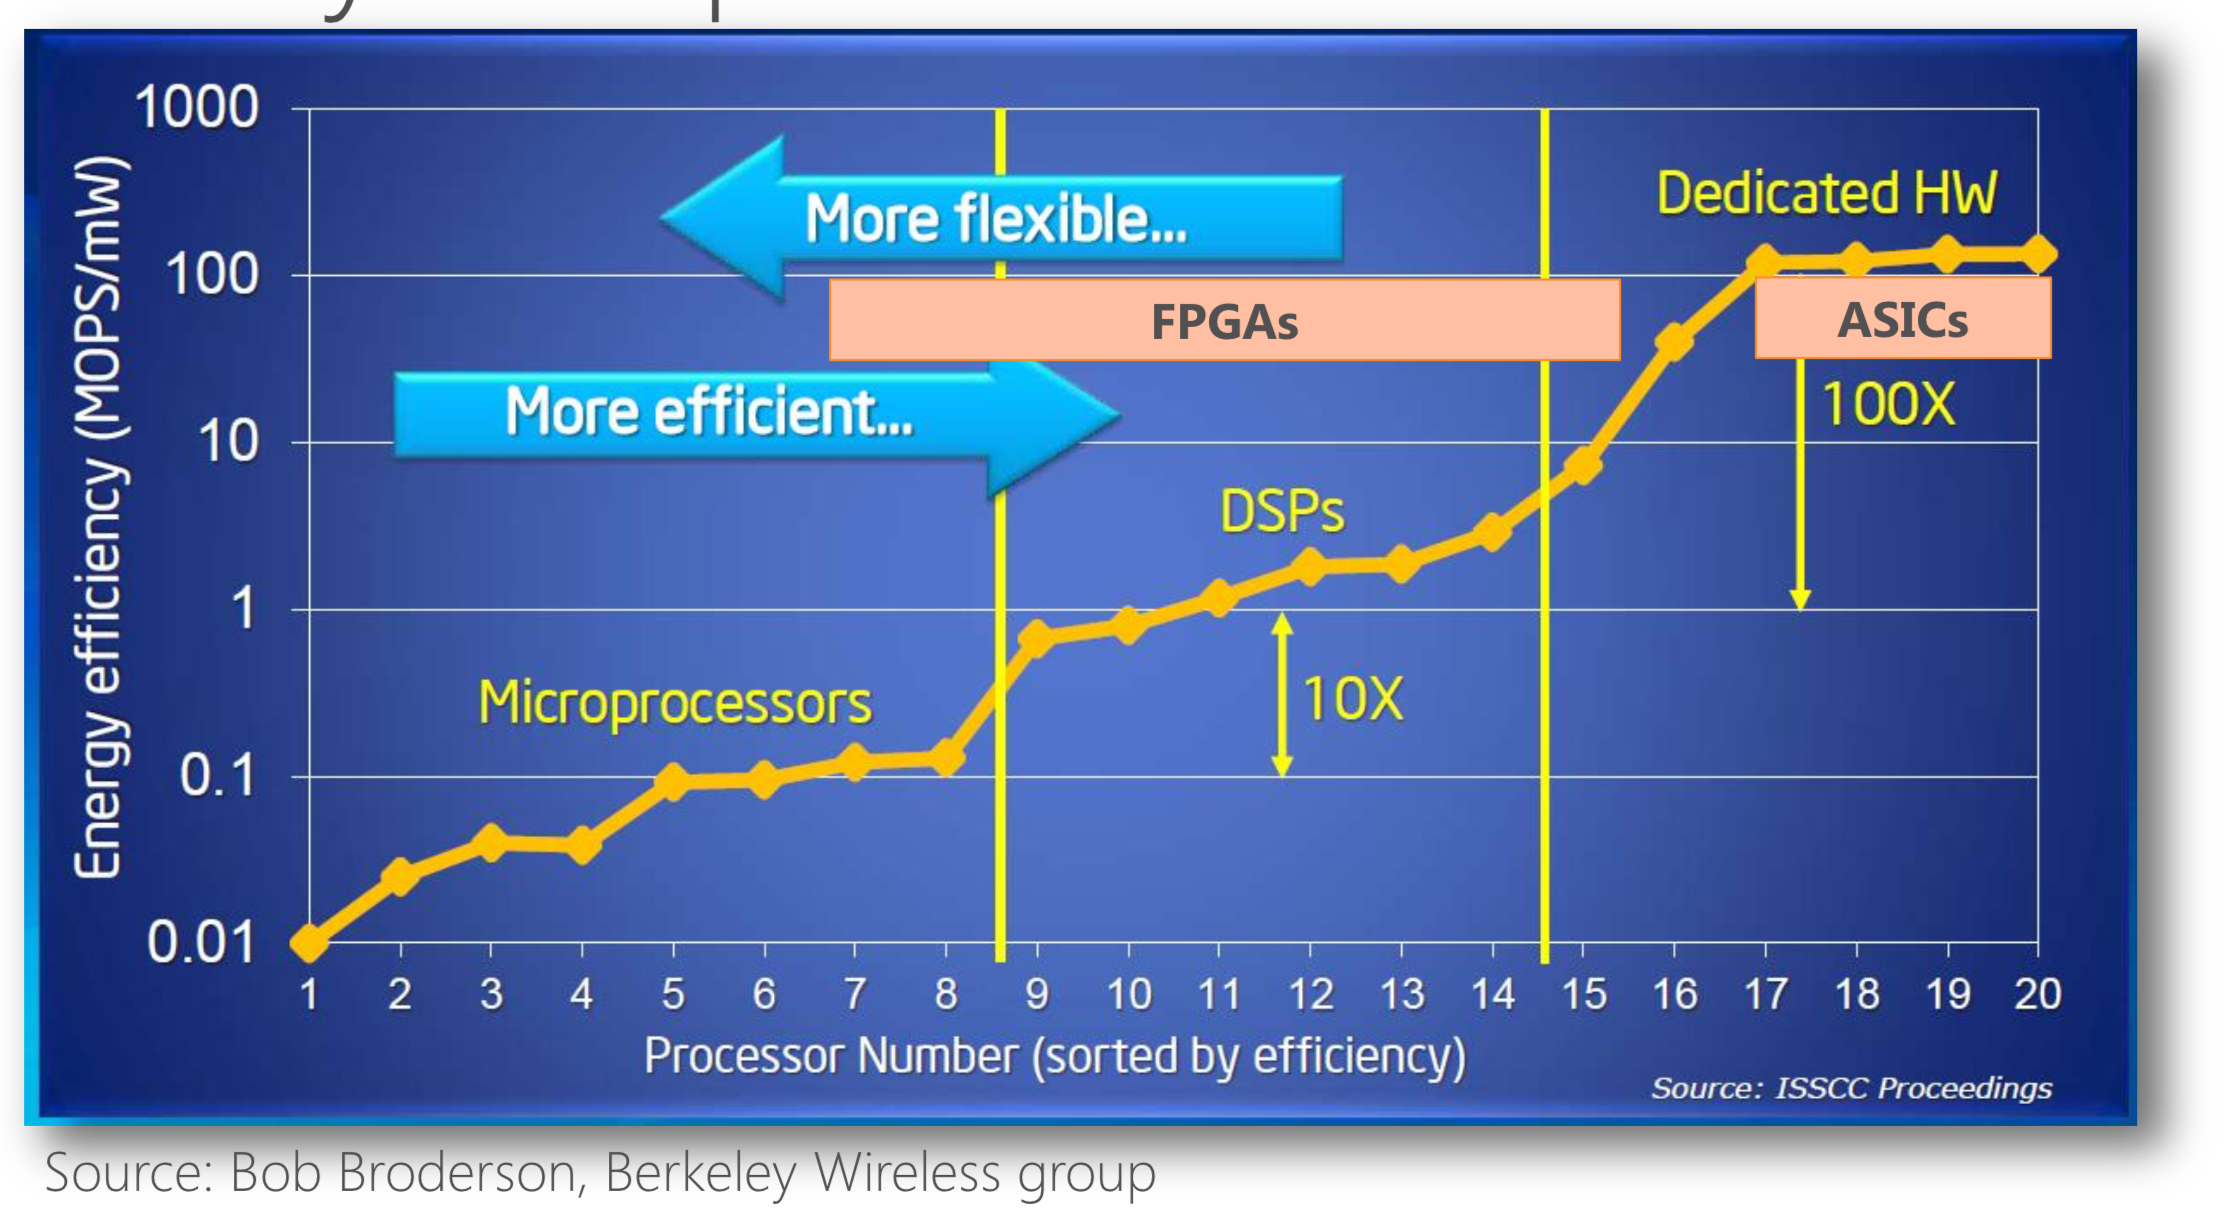
\includegraphics[width=10cm]{Figures/EfficiencyVSFlexibility.png}
	\caption[EfficiencyVSFlexibility]{Efficiency vs Flexibility}
	\label{fig:EfficiencyVSFlexibility}
\end{figure}

The whole development cycle shown in \emph{Figure} \ref{fig:FPGACycle} can be controlled using a high-level development language such as \emph{Xilinx's Vivado} GUI or Smalltalk as in \cite{XuanSang2014}. In the end, programming an FPGA consists of testing a design all the way through the process (with testbenchs and simulations) while performing a synthesis of the different components and deploying the resulting \emph{bitfile} on the hardware architecture.

% FPGA Development Cycle
\begin{figure}[htbp]
	\centering
		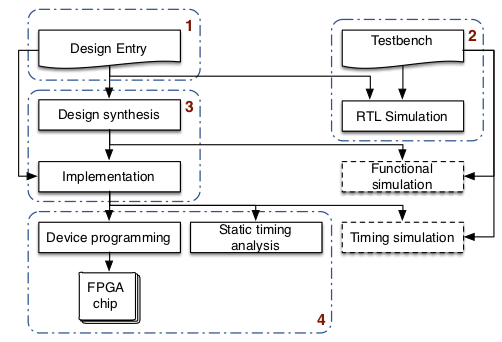
\includegraphics[width=10cm]{Figures/FPGACycle.png}
	\caption[FPGA Development Cycle]{FPGA Development Cycle \cite{XuanSang2014}}
	\label{fig:FPGACycle}
\end{figure}
